\chapter{Introduction}
\label{cha:intro}
\section{Importance of topic} \label{s:importance_topic}
''Society expects autonomous vehicles to be held to a higher standard than human drivers.'' \cite{Prof.Amnon} This quote sets the tone of the technology in autonomous driving. In order to be accepted by the public, autonomous vehicles should perform at least as reliable as conventional human drivers on parameters such as safety. Despite widespread research on self-driving vehicles, the acceptance by users stays limited.\cite{Bae2019} Research shows that purchase behaviour of customers can be directly linked with comfort. To gain more trust by the public it is clear that the challenge of making autonomous vehicles as comfortable as possible, should be tackled. This immediately leads to question: what is exactly comfort during driving?\\
Driving comfort is a personal experience and also depends on the emotional state of the driver. Therefore more than one driving style for an autonomous vehicle should be identified. \cite{Eindhoven2019} The state of the driver can be communicated to the vehicle at the start of each ride and different driving styles can be obtained by changing the parameters in a motion planning algorithm. 

\begin{figure}[h!]
	\centering
	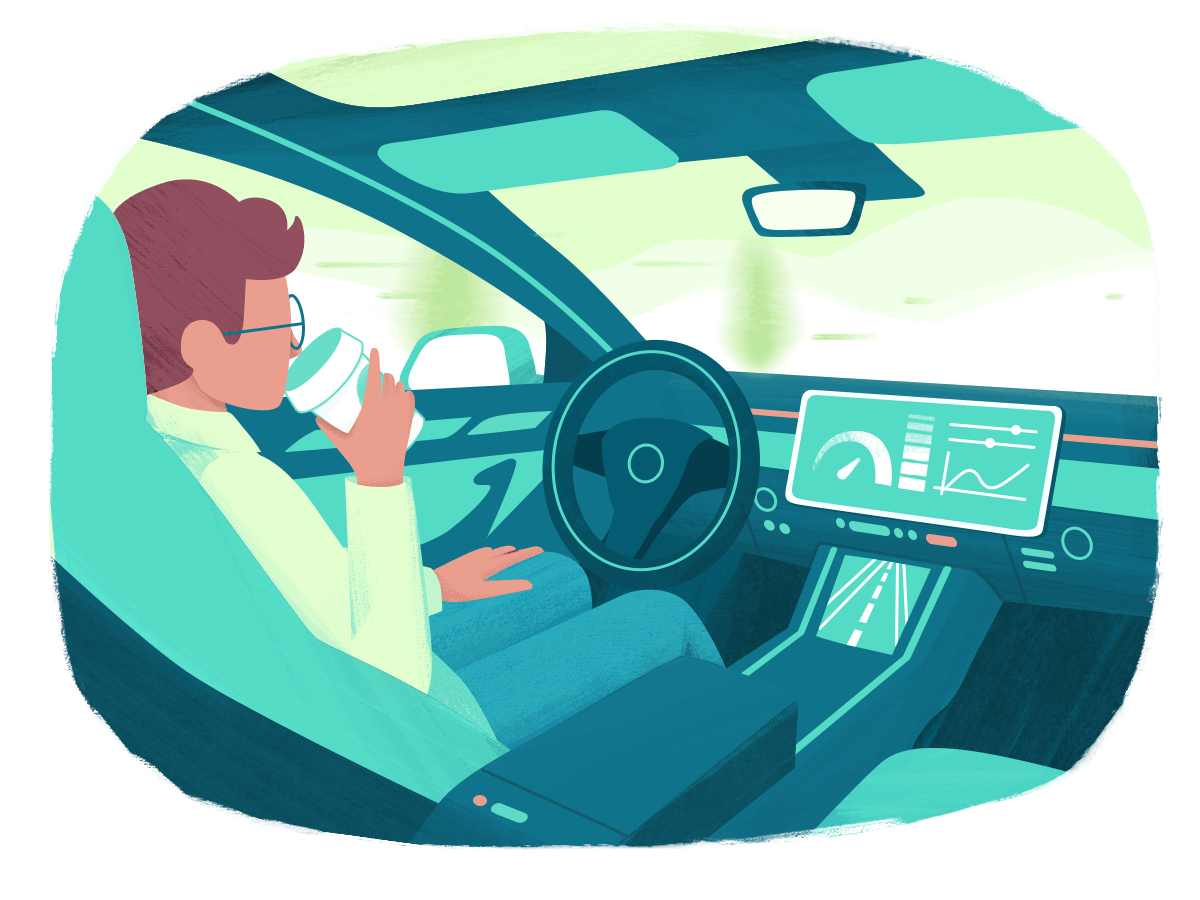
\includegraphics[width=0.50\linewidth]{AV}
	\caption{Concept visualization of autonomous driving. (source: \cite{AV})}
	\label{fig:AV}
\end{figure} 
\newpage

\section{Problem formulation and link with previous studies}
In order to identify specific comfort preferences of the driver that are quantified by parameters, the vehicle should be able to learn by demonstration. \cite{Kuderer2015a}\\
Despite that each driver has its own preferences, they are based on common comfort criteria where different trade-offs are made. For example, some drivers prefer a more aggressive driving style than others. This will manifest in a different set of parameters then the ones attained for a defensive driver for the same comfort criteria. The comfort criteria will later in this thesis be translated into an objective function where different weighting factors are used in order to quantify different comfort trade-offs made. In literature, this approach is called inverse optimal control or inverse reinforcement learning because it is learning the objective function for an optimal control problem.\\

In order to learn the weighting factors which can be used to distinguish different drivers, research about the common notion of comfort is necessary. Passenger surveys in public road transport about carsickness \cite{Turner1999} have identified lateral acceleration as the primarily responsible for motion sickness. It is explained that drive style is a main factor to influence the amount of sickness and it was found that sickness is higher when drivers drove with a higher average magnitude of fore-and-aft and lateral motion. These effects were far more significant than the effect of vertical vibrations. There is also a consensus reached about the contribution of continuous trajectories to the prevention of motion sickness and the natural feel of paths.\cite{Elbanhawi2015} This means that higher order kinematic variables like accelerations and jerks also should be considered when measuring comfort. Chapter \ref{cha:Literature_study} will give a more detailed description on the literature study conducted in order to investigate the state of the art comfort modelling. It will also discuss the theory of inverse optimal control.\\

\section{Thesis objective and structure}
The goal of this thesis is to build further on research of learning by demonstration as explained in \cite{Kuderer2015a} and to refine this idea by making use of more realistic vehicle models. Concretely the thesis is focussed on the implementation and validation of an algorithm that learns weighting factors in a comfort objective function which can explain observed driver data.\\
The learning process is done offline. After the different weighting factors are identified, the learned objective can be used to plan paths which can be followed by an autonomous vehicle, making use of an online tracking MPC.\\

The data used as observations is generated by simulations where it is assumed that the vehicle is driving on an straight at a speed range between $80\frac{km}{hours}$ and $100\frac{km}{hours}$. The maneuver investigated is a lane change maneuver as can be seen in Figure \ref{fig:lane_change}. In order to generate data, the non-linear bicycle and a more realistic $15$ dof of freedom Amesim model are used.\\

\begin{figure}[htp]
	\centering
	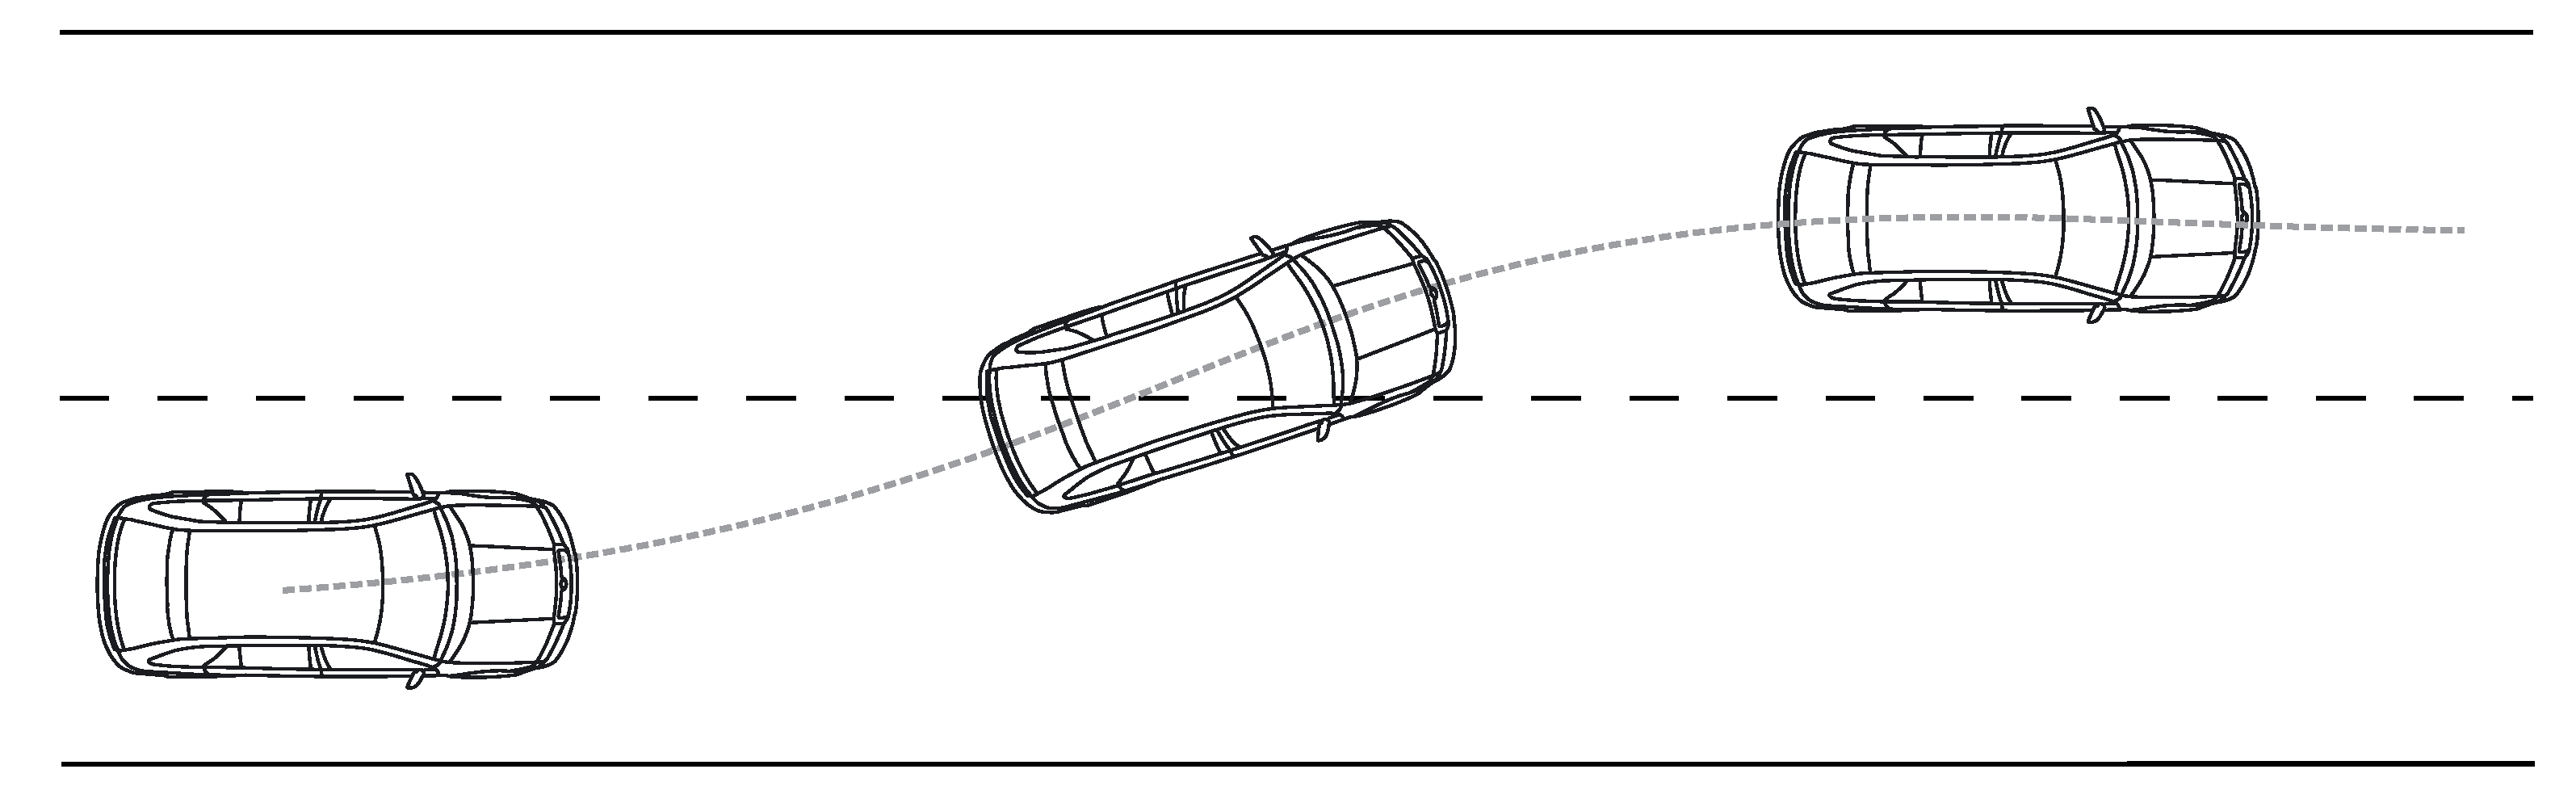
\includegraphics[width=0.8\textwidth]{lane_change.PNG}
	\caption{Example of a lane change which is the investigated maneuver in this thesis.}
	\label{fig:lane_change}
\end{figure}

The execution of this research was supported by "Siemens Digital Industries Software" located in Leuven which enabled a direct link with reality. Software was made available i.d. Simcenter Amesim.\\

The structure of the thesis is as follows. First, the reader is made acquainted with the optimal control concept in chapter \ref{cha:OCP}. The meaning is explained in section \ref{Optimal control problem (OCP)} and section \ref{s:MPC_e} gives an introduction to MPC. Next, chapter \ref{cha:Literature_study} discusses the state of the art modelling of comfort. This chapter is made out of 2 parts, section \ref{s:comfort_parameters} answers the question posed in section \ref{s:importance_topic}, explaining the meaning of comfort during driving. Section \ref{s:inverse re le} concerns a discussion on inverse optimal control concept. Chapter \ref{cha:Learning_algorithm} gives insight in learning from ideal data. The non-linear bicycle model is discussed in section \ref{sec:Vehicle_models} whereafter the formulation of the learning algorithm follows in section \ref{s:learning_alg}. Next, ideal data generation is analysed and validated in section \ref{s:GD}. Subsequently, different methods for learning from multiple datasets are discussed and results were analysed in section \ref{s:ID_results}. In chapter \ref{cha:Tracking_MPC} the non-linear bicycle model will be substituted by a more complex $15$ degrees of freedom Amesim model. First the flow of the learning algorithm is discussed in section \ref{s:flow of the algorithm}. Next the developed tracking MPC needed, is presented in section \ref{s:tracking_mpc}. Section \ref{s:complex_learning_results} gives an overview of the learning results. 
In chapter \ref{cha:Enhancement} the theoretical concept of an enhanced weight factor update method is proposed. Finally, chapter \ref{cha:conclusion} gives an general conclusion of this thesis.

%The reader is first given an introduction in the optimal control concepts whereafter  Next the learning from ideal data is discussed and the learning algorithm is validated by finding back initial chosen weighting factors. After this, the non-linear bicycle model used is substituted by a more complex $15$ degrees of freedom Amesim model. 

%To be able to make the generated data of high quality an MPC approach with a 15 degree of freedom vehicle model is used. Also in the learning algorithm itself a three degree of freedom non-linear bicycle model is used in order to adequately capture the different kinematic signals e.g. jerks and accelerations. Further there were comparisons made of different methods to learn from multiple datasets. \\

% Therefore the objective of this research is to develop an algorithm based on inverse reinforcement learning which is able to learn driver specific experiences of comfort during a lane change, captured in weighting factors of an objective function. Learning is done by looking at observations performed by the human driver because the learned objective function is an approximation of the one used when the driver generates comfortable paths. Comfort features, which are integrated kinematic vehicle signals in a formulation so that they determine a notion of comfort, are used in order to quantify similarity between observed and learned vehicle paths. The contribution of this thesis is to implement the theoretical idea of feature based learning with practical relevant vehicle models e.g. a $15$ degrees of freedom Amesim model. When the comfort objective is identified, it can be embedded in a path planning formulation for autonomous driving.\\

%%% Local Variables: 
%%% mode: latex
%%% TeX-master: "thesis"
%%% End: 
